\documentclass[utf8]{article}
\usepackage{amsmath,amssymb}
\usepackage{fancyhdr}
\usepackage{graphicx}
\usepackage{fullpage}
\usepackage{setspace}
\usepackage{fancyvrb}
\usepackage{geometry}
\usepackage{lastpage}
\usepackage{lipsum}
\geometry{left=2.5cm, right=2.5cm, top=2cm, bottom=4cm}

\title{\bf\LARGE AI+X Computing Acceleration: From Algorithms Development, Analysis, to Deployment: Final Report}
\author{Yuqi Ren 2022011332 \\ Jinfan Lu 2022010741}
\date{}

\pagestyle{fancy}
\fancyhf{}

\fancyhead[C]{Final Report}
\renewcommand{\headrulewidth}{0.2pt}
\setlength{\headsep}{1cm}

\fancyfoot[R]{Page \thepage\ of \pageref{LastPage}}
\renewcommand{\footrulewidth}{0.2pt}
\setlength{\footskip}{1.5cm}

\begin{document}
\maketitle
\thispagestyle{empty}

\section{Introduction}

In this project, we have implemented two advanced network topologies, SlimFly and DragonFly, alongside their corresponding routing algorithms and a deadlock-avoidance technique that utilizes virtual channels. SlimFly and DragonFly are among the most efficient topologies, with diameters of two and three, respectively.

...

\section{Architecture}
\subsection{Topology}
\begin{itemize}
    \item \textbf{SlimFly}: The SlimFly topology is characterized by a highly symmetric internal structure, consisting of two subgraphs, each composed of identical subgroups of routers. As depicted in Figure 1, the first subgraph consists of routers \((0,x,y)\), while the second is formed by routers \((1,m,c)\). These two subgraphs comprise \(q\) subgraphs that do not directly connect with each other, with each subgraph containing \(q\) routers. Router $(0, x, y)$ and router $(1, m, c)$ are connected if and only if $y = mx + c$.

    \begin{figure}[h]
        \centering
        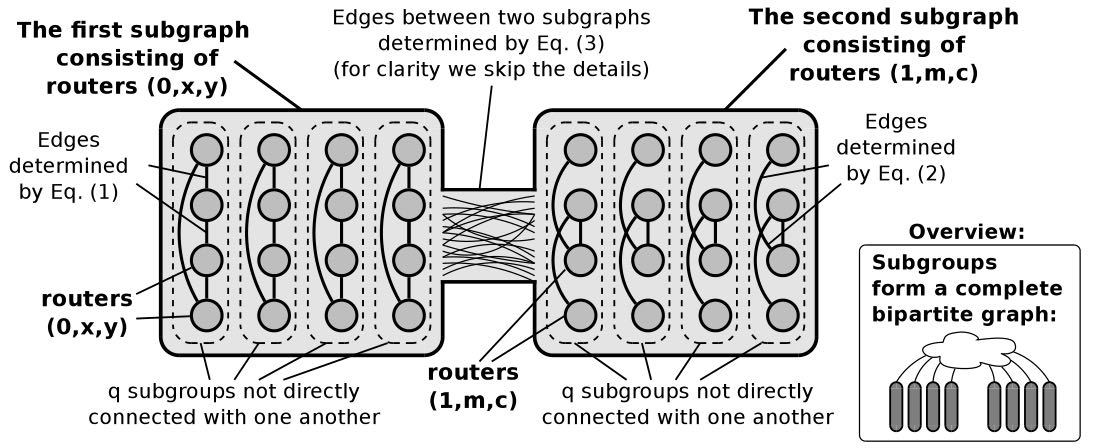
\includegraphics[width=0.7\linewidth]{SlimFly.png}
        \caption{SlimFly topology}
    \end{figure}

    Based on this topology, we can derive several key metrics: Diameter = \(2\), Degree = \(O(q)\), Average Distance \(\approx 2\), and Cost = \(O(q^3)\).

    \item \textbf{DragonFly}: The DragonFly topology is a hierarchical network organized into three levels: system, group, and router. At the group level, \(n\) routers within the same group are fully interconnected. At the system level, there are \(m\) groups, and each pair of groups is connected by a single link. Specifically, the \(i\)-th group and the \(j\)-th group are connected via global channels between the \((i \mathrm{~mod~} n)\)-th router in group \(j\) and the \((j-1 \mathrm{~mod~} n)\)-th router in group \(i\). From this topology, we can compute the following metrics: Diameter = \(3\), Degree \(\le n-1+\lceil m/n\rceil\), Average Distance \(\approx 3\), and Cost = \(O(n^2m)\). An example of a special DragonFly topology (\(m=2n+1\)) is shown in Figure 2.

    \begin{figure}[h]
        \centering
        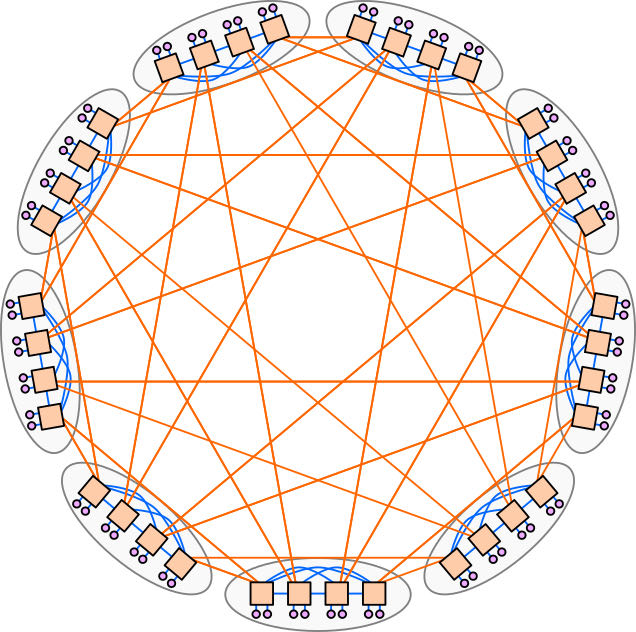
\includegraphics[width=0.4\linewidth]{DragonFly.png}
        \caption{DragonFly topology}
    \end{figure}
\end{itemize}

\subsection{Routing}
We have implemented two fundamental routing methods for the DragonFly and SlimFly topologies:
\begin{itemize}
    \item \textbf{Minimal Static Routing}: In minimal routing, a packet is forwarded along the shortest path from the source router \(R_s\) to the destination router \(R_d\).
    \item \textbf{Valiant Random Routing}: In Valiant routing, the protocol first randomly selects an intermediate router \(R_r\). The packet is then routed from the source router \(R_s\) to the intermediate router \(R_r\), and finally from \(R_r\) to the destination router \(R_d\). The resulting paths may consist of 2, 3, or 4 hops.
\end{itemize}

\subsection{Deadlock Freedom}
To ensure deadlock avoidance in SlimFly, we implement a technique that utilizes virtual channels. When sending a packet from router \(R_a\) to \(R_b\), if they are directly connected, virtual channel \(VC_0\) is used. Otherwise, as the maximum distance in SlimFly is two hops, virtual channel \(VC_0\) is used for the first hop and \(VC_1\) for the second hop. This approach effectively breaks cycles into different sets of buffers, thus preventing deadlocks.

\section{Implementation}

\subsection{Topology}
\begin{itemize}
    \item \textbf{SlimFly Topology}: The implementation of SlimFly involves two main steps: adding intra-group links and inter-group links. First, we divide routers into groups based on their indices. Then, we connect router \((0,x,y)\) with router \((0,x,y^\prime)\) if \(y-y^\prime \in X\), and connect router \((1,m,c)\) with router \((1,m^\prime,c^\prime)\) if \(c-c^\prime \in Y\), where \(X=\{1,\xi^2, \dots, \xi^{q-3}\}\), \(Y=\{\xi, \xi^3, \dots, \xi^{q-2}\}\), and \(\xi\) is an element of the Galois Field \(\mathbb{F}_q\) that generates \(\mathbb{F}_q\). Finally, we add inter-group links by connecting router \((0,x,y)\) with router \((1,m,c)\) if and only if \(y=mx+c\).

    In our implementation, considering a configuration with 64 CPUs, we set \(q=5\), resulting in 50 routers. Therefore, we have \(X = \{1, 4\}\) and \(X'=\{2, 3\}\).

    \item \textbf{DragonFly Topology}: The implementation of DragonFly follows a similar approach as SlimFly. We first add intra-group links and then inter-group links. Denoting the \(i\)-th router in group \(j\) as \((i,j)\), we add inter-group links as follows: connect router \((j-1 \mathrm{~mod~} n, i)\) with router \((i \mathrm{~mod~} n, j)\).
\end{itemize}

\subsection{Routing}
\begin{itemize}
    \item \textbf{Minimal Static Routing}: To find the shortest path, we assign a weight of 1 to all links in the network and use a shortest path algorithm.
    \item \textbf{Valiant Random Routing}: To select the intermediate router, we define a random selection mechanism that balances traffic.
\end{itemize}

\subsection{Deadlock Freedom}

In our implementation, we set the number of virtual channels to 2. When sending a packet, we check whether the destination router is directly connected. If it is, we use \(VC_0\); otherwise, we use \(VC_0\) for the first hop and \(VC_1\) for the second hop.

This modification mainly involves changes in \texttt{src/mem/ruby/network/garnet/OutputUnit.cc}, specifically in the logic for the functions \texttt{has\_free\_vc} and \texttt{select\_free\_vc}.

\section{Experiments and Analysis}

\subsection{Topology}

\subsection{Routing}

\subsection{Deadlock Freedom}

To evaluate the effectiveness of the deadlock-avoidance technique, we conducted simulations with and without the deadlock prevention algorithm. The built-in synthetic traffic patterns in Garnet are not suitable for detecting deadlocks in SlimFly, so we implemented a custom synthetic traffic pattern. In this pattern, most packets follow a specific path \((R_x, R_y)\), which is clearly illustrated below.

\begin{figure}[h]
    \centering
    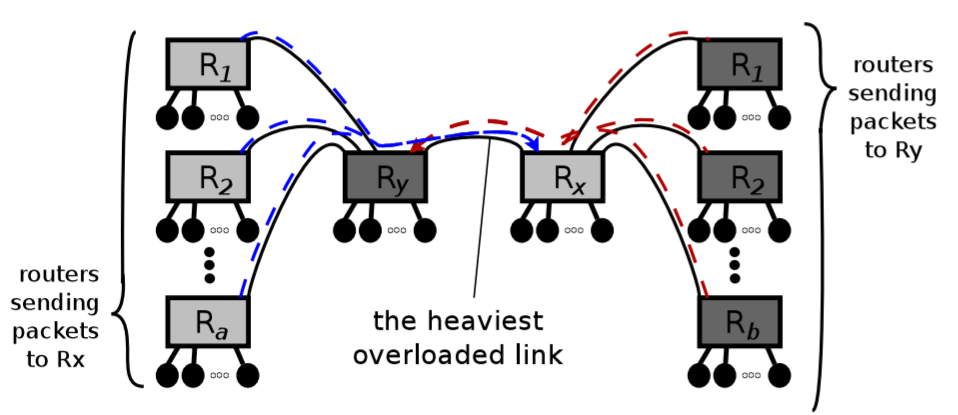
\includegraphics[width=0.5\linewidth]{WorstCase.png}
    \caption{Illustration of the worst-case scenario for SlimFly}
\end{figure}

\begin{figure}[h]
    \centering
    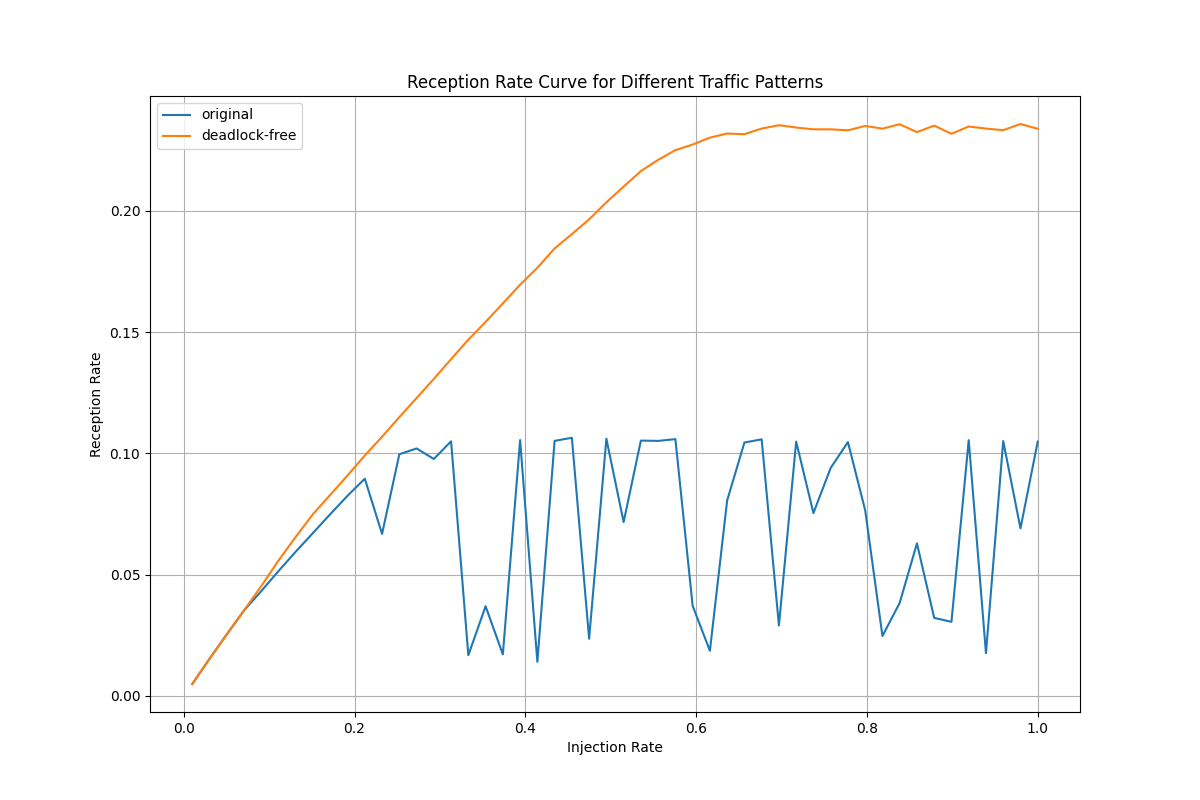
\includegraphics[width=0.5\linewidth]{deadlock.png}
    \caption{Experiemnts of deadlock free algorithm}
\end{figure}

We use reception rate to indicate the occurrence of deadlocks in the minimal static routing algorithm. The original algorithm shows some points with extremely low reception rates, indicating deadlocks. Due to the inherent randomness in our synthetic traffic pattern, some areas may still exhibit higher reception rates.

\section{Labor Distribution}
Yuqi Ren (50\%):
\begin{itemize}
    \item Paper reading
    \item DragonFly topology
    \item Minimal routing, Valiant random routing
    \item Experiments: deadlock
\end{itemize}

\end{document}
